\documentclass[11pt, addpoints, answers]{exam}
\usepackage[spanish]{babel}
\usepackage{amsmath}
\usepackage{amssymb}
\usepackage{graphicx}
\usepackage{tabularx}
\usepackage{ragged2e}
\usepackage{geometry}
\usepackage{booktabs}


% --- CONFIGURACIÓN DE PUNTUACIÓN EN ESPAÑOL  ---
% Definimos cómo se muestran los puntos: "punto" para singular y "puntos" para plural.

\pointpoints{punto}{puntos}

% --- AJUSTE DE MARGENES ---
\geometry{
	hmargin={1in, 1in},
	vmargin={1.2in, 1in},
}

% --- CONFIGURACIÓN DE PÁGINA Y ENCABEZADO FINAL ---
\pagestyle{headandfoot}

% 1. Definición Ultra-Robusta del Encabezado (soluciona Overfull \hbox)
\renewcommand{\firstpageheadrule}{%
	\dimen0=\tabcolsep
	\makebox[\textwidth]{%
		\hspace{-\dimen0}\makebox[\textwidth+2\dimen0]{%
			\textbf{Nombre del estudiante:} \enspace\hrulefill \hspace{2em}
			\textbf{Grupo:} \enspace\hrulefill
		}%
	}\vspace{1ex}\hrule
}

% 2. Define el contenido del encabezado de la universidad (centrado)
\firstpageheader{}{\centering\textbf{Examen Diagnóstico de Matemática}\\\textbf{Universidad Estatal Guayaquil}}{}

% 3. Define el pie de página
\firstpagefooter{}{Página \thepage\ de \numpages}{}
\runningheader{Diagnóstico Matemática}{}{Pág. \thepage}
\runningfooter{}{}{}

\begin{document}
% --- NUEVA SECCIÓN PARA DATOS DEL ALUMNO ---
% Usamos \makebox para alinear el Nombre a la izquierda y el Grupo a la derecha.
\makebox[\textwidth]{
	\textbf{Nombre:} \enspace\hrulefill \hspace{4em}  
	\textbf{Grupo:} \enspace\hrulefill 
}


	
	\vspace{0.5cm}
	
	% -------------------------------------------------------------
	% COMIENZA EL EXAMEN (Todas las preguntas)
	% -------------------------------------------------------------
	\begin{questions}
		
		% La puntuación aquí saldrá en rojo. Ejemplo: [1 punto]
		\question[1] \textbf{Resuelve las siguientes ecuaciones.} 
		
		\begin{parts}
			\part $x^2 + 4 = 0$
			\part $3x + 4x - 2x = 8$
			\part $4x - 32 = 5x + 13$
			\part $2x + 1 = 8$
		\end{parts}
		
		% PREGUNTA 2: ÁNGULOS (Múltiple Opción)
		\question[1] \textbf{¿Qué ángulos son iguales al ángulo 6 de la figura?}
		\begin{center}
			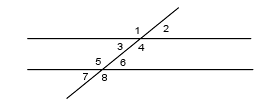
\includegraphics[width=0.4\textwidth]{image_243168.png}
		\end{center}
		\begin{choices}
			\choice 2, 3 y 5
			\choice 2, 3 y 7
			\choice 5, 7 y 2
			\choice 1, 4 y 7
		\end{choices}
		
		% PREGUNTA 3: SÍMBOLOS DE AGRUPACIÓN
		\question[1] \textbf{Elimine los símbolos de agrupación y reduzca términos semejantes.}  
		\begin{parts}
			\part $17 - 7(3x - 4)$
			\part $2(5x - 4y) - (7x + y)$
			\part $x - [7 - 3(2x - 4)]$
			\part $(2x - 3y) - 4(x - 5y)$
		\end{parts}
		
		% PREGUNTA 4: FACTORIZACIÓN
		\question[1] \textbf{Factorizar los siguientes polinomios.}  
		\begin{parts}
			\part $4(x-3)^2 + 6(x-3)$
			\part $9a^2 - 4$
			\part $x^2 + 8x + 15$
			\part $2x^2 + 9x + 4$
		\end{parts}
		
		% PREGUNTA 5: FRACCIONES ALGEBRAICAS (VERTICAL Y CON PUNTUACIÓN AJUSTADA)
		\question[1] \textbf{Señale la respuesta correcta:}
		
		\textbf{5.1 (0.5 pts): Si sumamos las fracciones $\frac{4}{x+2} + \frac{2x}{x+2}$ dará por resultado:}
		
		\begin{choices} % CAMBIADO a choices para opciones verticales
			\choice $\frac{6x}{x+2}$
			\choice $\frac{4+2x}{x+2}$
			\choice $\frac{4+2x}{(x+2)^2}$
			\choice 2
		\end{choices}
		
		\vspace{1cm}
		
		\textbf{5.2 (0.5 pts): Si sumamos $\frac{x}{x+3} + \frac{2}{x-2}$ su resultado será:}
	
		\begin{choices} % CAMBIADO a choices para opciones verticales
			\choice $\frac{2x}{(x+3)(x-2)}$
			\choice $\frac{2x}{2x+5}$
			\choice $\frac{x^2+6}{(x+3)(x-2)}$
			\choice $\frac{1}{6}$
		\end{choices}
		
		% PREGUNTA 6: SISTEMA DE ECUACIONES
		\question[1] \textbf{El conjunto solución del sistema $\begin{cases} 3x+2y=7 \\ 2x+5y=12 \end{cases}$ es:}
		\begin{choices}
			\choice $(1, 2)$
			\choice $(-1, 2)$
			\choice $(1, -2)$
			\choice $(2, 1)$
		\end{choices}
		
		% PREGUNTA 7: RECTA
		\question[1] \textbf{Considerando la siguiente gráfica, la ecuación de la recta sería:}
		\begin{center}
			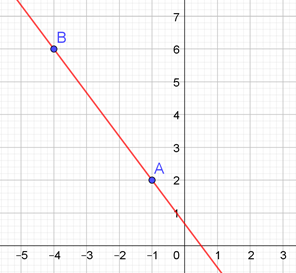
\includegraphics[width=0.6\textwidth]{image_248acc.png}
		
		\end{center}
		\begin{choices}
			\choice $y-3 = \frac{4}{3}x+6$
			\choice $y = 5x-2$
			\choice $y-2 = -\frac{4}{3}x - \frac{4}{3}$
			\choice $y = -\frac{1}{3}x+2$
		\end{choices}
		
			\vspace{1.5cm}
		
		% PREGUNTA 8: PROPIEDADES DE POTENCIAS
		
		\question[1] \textbf{¿Cuál de las siguientes igualdades es correcta?}
		\begin{choices}
			\choice $7^2 \cdot 7^4 \cdot 7 = 7^6$
			\choice $7^2 \cdot 7^{-1} \cdot 7^3 = 7^4$
			\choice $7^2 + 7^4 + 7 = 21^7$
			\choice $7^2 + 7^{-1} + 7^3 = 7^3$
		\end{choices}
		
		% PREGUNTA 9: FUNCIÓN
		\question[1] \textbf{Selecciona cuál de las siguientes reglas de correspondencia pertenece a la función representada.}
		\begin{center}
			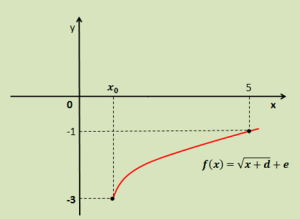
\includegraphics[width=0.5\textwidth]{image_249683.png}
		\end{center}
		\begin{choices}
			\choice $f(x) = \sqrt{x-5}-1$
			\choice $f(x) = \sqrt{x-1}-3$
			\choice $f(x) = \sqrt{x+1}-3$
			\choice $f(x) = \sqrt{x-1}+3$
		\end{choices}
		
		% PREGUNTA 10: RELACIONAR COLUMNAS (Tabla)
		\question[1] \textbf{Escribe en la Columna B los resultados correspondientes a cada una de las operaciones de la Columna A.}
		\v
		
		\begin{tabularx}{\textwidth}{|>{\RaggedRight\arraybackslash}X|X|}
			\hline
			\textbf{Columna A (Operación)} & \textbf{Columna B (Resultado)} \\
			\hline
			$\left(\left(\left(\frac{1}{2}\right)^3\right)^0\right)^{-2}$ & \\
			\hline
			$(6x^2+13x-5) \div (3x-1)$ & \\
			\hline
			$\sqrt[3]{9x^6 \cdot x^8}$ & \\
			\hline
			$\frac{3}{4} = \frac{9}{?}$ & \\
			\hline
			$\log(100) - \log(10)$ & \\
			\hline
		\end{tabularx}
		
	\end{questions}
\end{document}